\documentclass{article}[11pt]
\usepackage{graphicx}
\usepackage{float}

\title{ERSMS, Group F, Project Documentation}
\author{Hubert Dwornik, Michał Łezka, Jakub Mazur \\ Michał Sar, Krzysztof Rudnicki}
\begin{document}
\maketitle

\section{System Architecture} 
We have designed and implemented 4 microservices,
all of microservices are written in Python using Flask framework
\paragraph{AI recommendations}
Based on a list of movies ids, calculates and returns list of ids recommended for user who likes given movies
\paragraph{Analytics}
Holds information about number of 
ratings, number of users, 
average movie ratings, ratings of 
given user which are later used in 
webinterface to show data for admins 
concerning website usage
\paragraph{Notifications}
Notifies user whenever there is a new movie recommend by AI recommender for them 
\paragraph{Backend}
Updates database and mantains all ongoing and incoming communication between all microservices, both between microservies and from microservices to the webinterface
\paragraph{Caching}
We implemented two caches
\begin{enumerate}
    \item Backend is cached inside Analytics Service \\
    Analytics service holds tata about users and movies, 
    in order to not pull all the data from backend every time we update analytics
    (for example every day), we keep the cache of backend date in our analytics 
    service
    \item AI recommendations are cached inside Notification Service \\ 
    AI recommendations can change whenever new movie appears, notification 
    service keeps the cache of ai recommendation service in order to not 
    pull all the data from the ai recommendation every time it wants to notify 
    the users about new movies to recommend
\end{enumerate}
\paragraph{Database}
We use postgresql database to contain data about users, movies and user ratings


\begin{figure}[H]
    \caption{System architecture representation, webinterface although not part of microservices included to show relation with backend}
    \centering
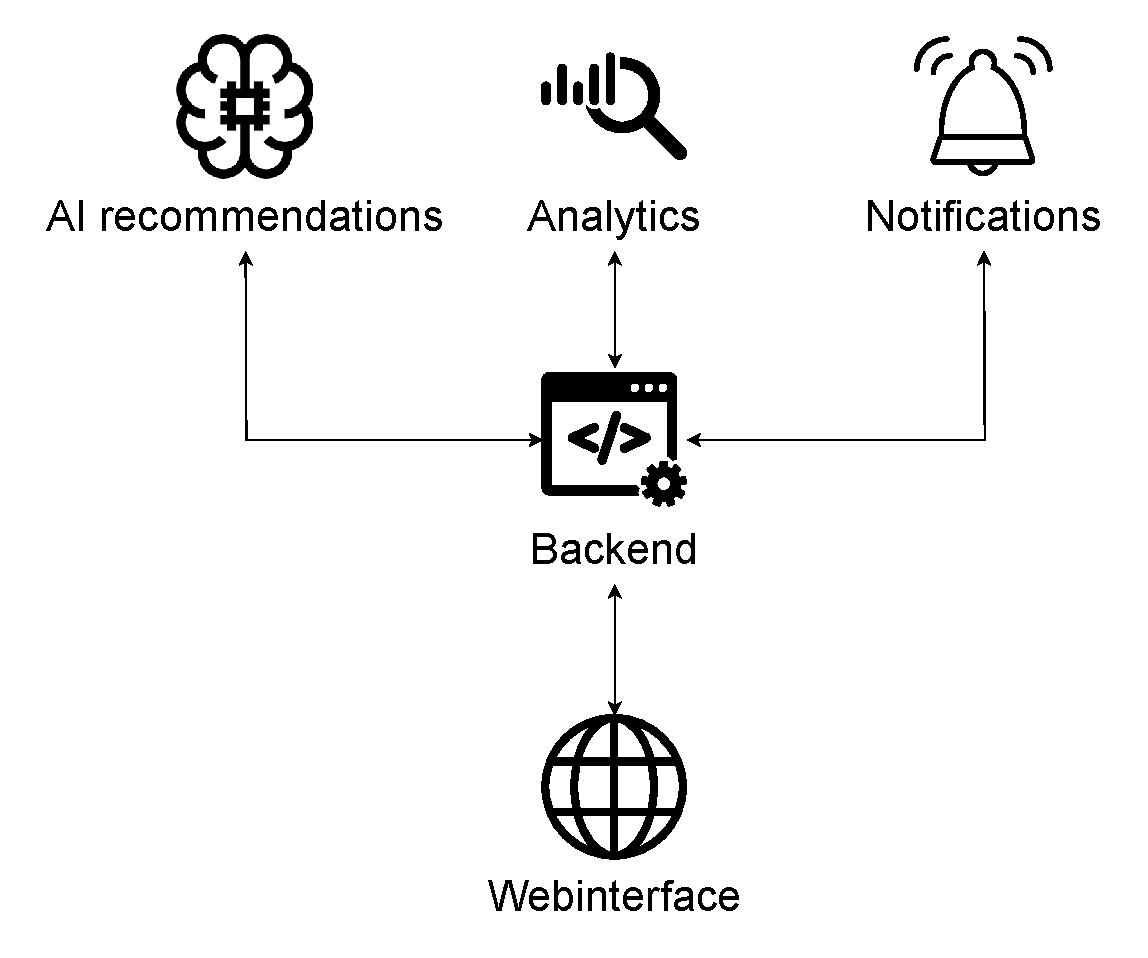
\includegraphics[width=\textwidth]{images/systemArchitecture.drawio.pdf}
\end{figure}


\section{Automated Infrastructure Management solution}
We use \textbf{Dockerfiles}
for each microservice, webinterface and database which 
later get combined in docker compose file, after each commit on 
\textbf{GitHub} main repository docker compose gets automatically run 
on \textbf{Google Cloud} platform and deployed 
\section{Federated authorization and authentication management in the project}
We use industry standard \textbf{OAuth} protocol in our webinterface, 
user creates their account and logs in, we use user token to 
authorize their access on backend to their ratings and 
recommendations. We use \textbf{firebase} services to manage OAuth protocol.
\section{Threat model with mitigations}
Our single most important asset are user likes for specific movies \\ 
We expect either bots or human agents trying to access those likes for a specific users or to modify user ratings to improve or decrease certain movies ratings \\ 
To mitigate that we use: 
\begin{enumerate}
    \item Certificates on our frontend, which encrypt data transmitted between website and user 
    \item OAuth which is used to authenticate user and lower amount of bots accessing our Infrastructure
    \item TLS encryption between our microservices so that even our inside communication is encrypted 
    \item Google cloud default security policies allowing us to monitor odd and potentially harmfull behaviours
\end{enumerate}
\begin{figure}[H]
    \caption{Threat model}
    \centering
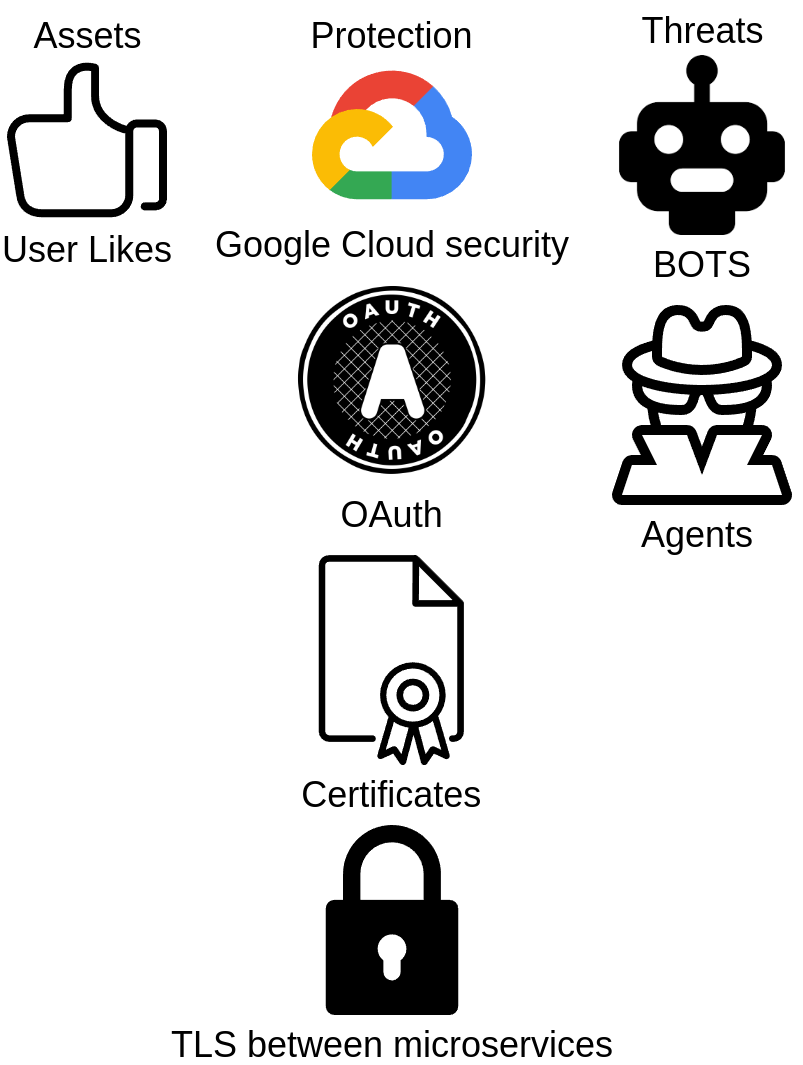
\includegraphics[width=\textwidth]{images/threat_model.png}
\end{figure}


\end{document}